% !Mode:: "Tex:UTF-8"


\section{Tipos de Variables.}
\label{cap01:sec:TiposVariables}

%\subsection*{Contenido:}
%\begin{itemize}
% \item Variables cualitativas y cuantitativas.
% \item Variables cuantitativas discretas y continuas.
% \item Notación para las variables. Frecuencia.
%\end{itemize}
  A lo largo del curso estudiaremos técnicas para describir y/o analizar
características de una población. Los datos que obtengamos los almacenaremos en
variables. Podemos pensar en una variable como una especie de
``contenedor'' en el que guardar los datos. Dependiendo del tipo de
característica en la que estemos interesados, usaremos un tipo de variable u
otro para almacenar la información a partir de la que empezar a trabajar.

\subsection{Variables cualitativas y cuantitativas.}
\label{cap01:subsec:VariablesCualitativasCuantitativas}

A veces se dice que las variables cuantitativas son las variables
numéricas,
	  y las cualitativas las no numéricas. La diferencia es, en realidad,
	 un poco más sutil. Una variable es {\sf cualitativa nominal}
	  \index{variable cualitativa nominal} cuando {\sf sólo} se utiliza para
	  establecer categorías, y {\em no para hacer operaciones con ella}. Es
decir, para poner nombres, crear clases o especies dentro de los individuos que
estamos estudiando. Por ejemplo, cuando clasificamos a los seres vivos en
especies, no estamos {\em midiendo nada}. Podemos {\em representar} esas
especies mediante números, naturalmente, pero en este caso la utilidad de ese
número se acaba en la propia representación, y en la clasificación que los
números permiten. Pero no utilizamos las propiedades de los números (las
operaciones aritméticas, suma, resta, etc.).
	Volviendo al ejemplo de las especies, no tiene sentido sumar especies de
seres vivos. A menudo llamaremos a estas variables {\sf
factores}\index{factor}, y diremos que los distintos valores que puede tomar un
factor son los {\sf niveles}\index{niveles de un factor} de ese factor. Por
ejemplo, en un estudio sobre c\'omo afecta al crecimiento de una planta el tipo
de riego que se utiliza, podríamos utilizar un factor (variable cualitativa)
llamado {\em riego}, con niveles: {\em ninguno, escaso, medio, abundante}.

Una {\sf variable cuantitativa}, \index{variable cuantitativa} por el
contrario,
	  tiene un valor numérico, y las operaciones matemáticas que se pueden
hacer con ese número son importantes para nosotros. Por ejemplo, podemos medir
la presión arterial de un animal y utilizar fórmulas de la mecánica de fluidos
para estudiar el flujo sanguíneo.

En la frontera, entre las variables cuantitativas y las cualitativas,
se incluyen las {\sf cualitativas ordenadas}\index{variable cualitativa
ordenada}. En este caso existe una ordenación dentro de los valores de la
variable.
\begin{ejemplo}
\label{cap01:ejem:VariableCualitativaOrdenada}
Un ejemplo de este tipo de variables es la gravedad del pronóstico de un enfermo ingresado en un
hospital. Como ya hemos dicho, se pueden codificar mediante números de manera que el orden se corresponda con el de los códigos numéricos, como aparece en la Tabla \ref{cap01:tabla:EjemploVariableCualitativaOrdenada}.
\begin{table}[h!]
        \begin{center}
        \begin{tabular}{|c|c|}
        \hline
        {\em Pronóstico}&{\em Código}\\
        \hline
        Leve&1\\
        \hline
        Moderado&2\\
        \hline
        Grave&3\\
        \hline
        \end{tabular}
        \end{center}
\caption{Un ejemplo de variable cualitativa ordenada.}
\label{cap01:tabla:EjemploVariableCualitativaOrdenada}
\end{table}

Pero no tiene sentido hacer otras operaciones con esos valores: no
podemos sumar grave con leve.
\qed
\end{ejemplo}

En este caso es {\em especialmente importante} no usar esos números para
operaciones estadísticas que pueden no tener significado (por ejemplo, calcular
la media, algo de lo que trataremos en el próximo capítulo).


\subsection{Variables cuantitativas discretas y continuas.}
\label{cap01:subsec:VariablesCuantDiscretasContinuas}


A su vez, las variables cuantitativas (aquellas con las que las operaciones numéricas tienen sentido) se dividen en \index{variable
discreta}\index{variable continua}\index{continua, variable}\index{discreta, variable} {\sf discretas} y {\sf continuas}. Puesto
que se trata de números, y queremos hacer operaciones con ellos, la
clasificación depende de las operaciones matemáticas que vamos a realizar.

Cuando utilizamos los {\sf números enteros} ($\mathbb Z$), que son
\[\ldots,-3,-2,-1,0,1,2,3,\ldots \]
o un subconjunto de ellos como modelo, la variable es discreta. Y entonces con esos
números podemos sumar, restar, multiplicar (pero no siempre dividir).

Por el contrario, si usamos {\sf los números reales} ($\mathbb R$),
entonces la variable aleatoria es continua. La diferencia entre un tipo de datos
y el otro se corresponde en general con la diferencia entre digital y analógico.
Es importante entender que la diferencia entre discreto y continuo es,
en general, una diferencia que establecemos nosotros al crear un {\sf
modelo} con el que estudiar un fenómeno, y que la elección correcta, entre otras cosas, del tipo de variable, determina la
utilidad del modelo. Un ejemplo clásico de este tipo de situaciones es el uso de la variable {\em tiempo}. Cuando alguien nos dice que una
reacción química, por ejemplo la combustión en un motor diesel a 1500 rpm, ha transcurrido en 5.6 milisegundos, está normalmente claro que, en el
contexto de este problema, nos interesan los valores de la variable tiempo con mucha precisión, y la diferencia entre 5.6 y, por ejemplo, 5.9
milisegundos puede ser fundamental. Además, y aún más importante, en este tipo de situaciones, damos por sentado que la variable tiempo podría tomar
{\em cualquier valor en un cierto intervalo}. Si observáramos esa reacción con aparatos más precisos, a lo mejor podríamos decir que el tiempo de la
combustión es de 5.57 milisegundos, y no, por ejemplo, de 5.59 milisegundos. {!`}Aunque, por supuesto, ambas cantidades se redondearán a 5.6 milisegundos
cuando sólo se usan dos cifras significativas!\footnote{Hablaremos con detalle sobre cifras significativas en la Sección \ref{cap01:sec:PrecisionExactitudCifrasSignificativas}} Por el contrario, si decimos que el tratamiento de un paciente en un hospital ha durado
tres días, está claro que en el contexto de este problema no queremos decir que el paciente salió por la puerta del hospital exactamente 72 horas (o
259200 segundos) después de haber entrado. El matiz esencial es que {\em no nos importa la diferencia} entre salir a las 68 o a las 71 horas. Y
decidimos usar una unidad de tiempo, el día, que {\em sólo toma valores enteros, separados por saltos de una unidad.} En este problema hablamos de un
día, dos o tres días, pero no diremos que el paciente salió del hospital a los 1.73 días. Eso no significa que no tenga sentido hablar de 1.73 días.
{!`}Naturalmente que lo tiene! La  cuestión es si nos importa, si necesitamos ese nivel de precisión en el contexto del problema que nos ocupa.\\

Somos conscientes de que esta diferencia entre los tipos de variables y su uso en distintos problemas es una cuestion sutil, que
sólo se aclarará progresivamente a medida que el lector vaya  teniendo más experiencia con modelos de los diversos tipos: discretos,
continuos, y también factoriales. Además este tema toca de cerca varias cuestiones (como la idea de precisión, o el uso de las cifras significativas)
sobre los que volveremos más adelante, en la Sección \ref{cap01:sec:PrecisionExactitudCifrasSignificativas}, y siempre que tengamos ocasión a lo largo del curso.


\subsection{Notación para las variables. Tablas de frecuencia. Datos agrupados.}
\label{cap01:subsec:NotacionVariablesTablasFrecuenciaDatosAgrupados}

En cualquier caso, vamos a tener siempre una lista o {\sf vector}\index{vector de datos (observaciones, medidas)} $x$ de valores
(datos, observaciones, medidas) de una variable, que representaremos con símbolos como
    \[x_1,x_2,\ldots,x_n\mbox{ o también }x=(x_1,x_2,\ldots,x_n)\]
    El {\sf número $n$} se utiliza habitualmente en Estadística para referirse
al {\sf número total de valores} de los que se dispone.
Por ejemplo, en el fichero
%\textattachfile{../fig/cap01-DatosAlumnos.csv}{\textcolor{
%blue}{cap01-DatosAlumnos.csv}}
\fichero{../datos/cap01-DatosAlumnos.csv}{cap01-DatosAlumnos.csv}
(hay una versión adecuada para usarla en la hoja de cálculo Calc, usando comas para los decimales:
\fichero{../datos/cap01-DatosAlumnos-Calc.csv}{{cap01-DatosAlumnos-Calc.csv}}) tenemos una tabla con datos de  los 100 alumnos de una clase ficticia. No te preocupes de los detalles técnicos del fichero, por el momento. En los primeros  tutoriales del curso explicaremos  cómo
usar este fichero con el ordenador. Para cada alumno tenemos, en una fila de la tabla, un valor de cada una de las variables {\em género, peso , altura ,
edad}.  En la Figura \ref{cap01:fig:DatosAlumnosCalc} se muestra una parte de los datos que contiene este fichero, abierto con la hoja de cálculo Calc.

    \begin{figure}[h]
	\begin{center}
	\begin{enColor}
% 	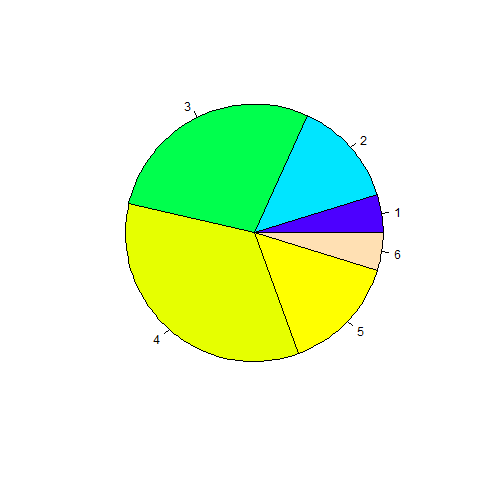
\includegraphics[height=6cm]{../fig/Cap01-DiagramaSectores.png}
% 	\hspace{0.5cm}
	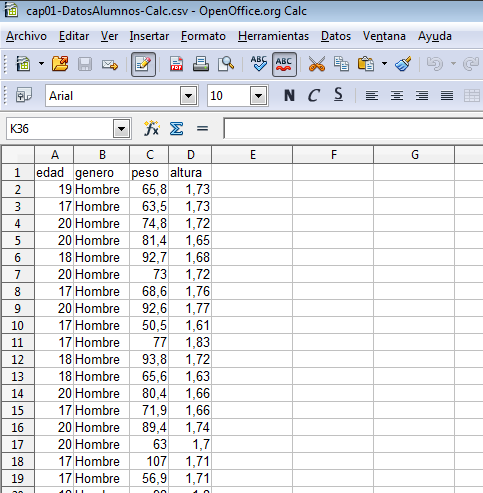
\includegraphics[height=7cm]{../fig/Cap01-DatosAlumnos.png}
	\end{enColor}
	\begin{bn}
% 	\includegraphics[height=6cm]{../fig/Cap01-DiagramaSectores-bn.png}
% 	\hspace{0.5cm}
	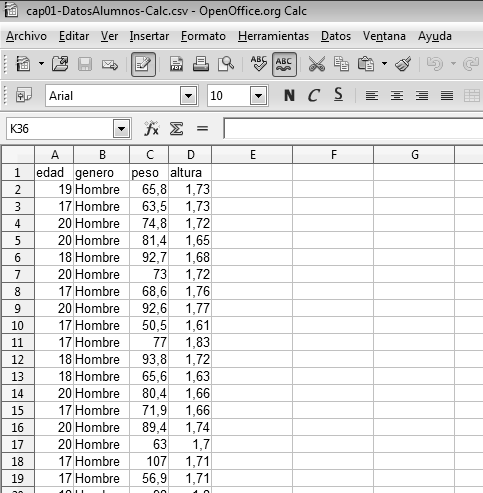
\includegraphics[height=7cm]{../fig/Cap01-DatosAlumnos-bn.png}
	\end{bn}
	\caption{El contenido del fichero {\tt cap01-DatosAlumnos.csv}, en Calc.}
	\label{cap01:fig:DatosAlumnosCalc}
    \end{center}
    \end{figure}


Vamos a utilizar estos datos para ilustrar algunas de las ideas que iremos viendo.

Una observación: si utilizamos $p_1,p_2,\ldots,p_{100}$ para referirnos, por ejemplo, a los datos de peso de esa tabla,
entonces $p_1$ es el dato en la segunda fila, $p_2$ el dato en la tercera, y
$p_{35}$ el dato de la fila $36$. Porque, como veremos, puede ser
cómodo y conveniente conservar los nombres de las variables en la primera fila
de la tabla de datos. Además, en estos casos puede ser una buena idea
introducir una columna adicional con el índice $i$ que corresponde a $p_i$ ($i$
es el número de la observación).

Un mismo valor de la variable puede aparecer repetido varias veces en
la serie de observaciones. En el fichero de alumnos del que estamos
hablando, la variable {\em edad} toma estos cuatro valores distintos:
\[17,\qquad  18,\qquad 19,\qquad 20\]
Pero, naturalmente, cada uno de esos valores aparece repetido unas cuantas veces; no en vano {!`}hay 100 alumnos! Este {\sf número de repeticiones de un
valor} es lo que llamamos la {\sf frecuencia} \index{frecuencia} de ese valor. Por ejemplo, el valor 20 aparece repetido 23 veces, lo que significa
obviamente que hay 23 alumnos de 20 años de edad en esa clase. ¿Cómo hemos sabido esto? Desde luego, no los hemos contado ``a mano''. Una de las
primeras cosas que haremos en los tutoriales del curso es aprender a obtener la frecuencia en un caso como este.


% , {\em Hombre} o {\em Mujer} (es una
% variable cualitativa o factor, con dos niveles). Pero cada uno de esos valores
% aparece repetido bastantes veces. En concreto en la clase hay 57
% alumnos y 35 alumnas.

El número de repeticiones de un valor, del que hemos hablado en el anterior párrafo, se llama {\sf frecuencia absoluta}\index{frecuencia
absoluta}, para distinguirlo de la {\sf frecuencia relativa}\index{frecuencia relativa}, que se obtiene dividiendo la frecuencia absoluta por $n$ (el
total de observaciones). La frecuencia relativa es un {\em tanto por uno}, y se convierte fácilmente en un {\sf porcentaje}\index{porcentaje y
frecuencia relativa}, multiplicándola por 100. Volveremos sobre este tema en el Capítulo \ref{cap:ValoresCentralesDispersion} (ver la página \pageref{cap02:subsubsec:MedianaTablasFrecuenciasRelativasAcumuladas}).
%\fernando{¿Cuándo nos conviene hablar de frecuencias acumuladas? Yo creo que mejor en el segundocapítulo...}


Cuando tratamos con variables cualitativas o discretas, muchas veces, en lugar del valor de cada observación la información que tenemos es la
de las frecuencias de cada uno de los posibles valores distintos de esas variables. Esto es lo que se conoce como una {\sf tabla de
frecuencias}\index{tabla de frecuencias}. Por ejemplo, la Tabla \ref{cap01:tabla:FrecuenciaEdadClase} (pág.\pageref{cap01:tabla:FrecuenciaEdadClase})
es la tabla de frecuencia de la variable edad en este ejemplo

\begin{table}[ht]
\centering
\begin{tabular}{cc}
  \hline
  edad& frecuencia \\
  \hline
  17 &  17 \\
  18 &  37 \\
  19 &  23 \\
  20 &  23 \\
   \hline
\end{tabular}
\caption{Tabla de frecuencia. variable edad en el ejemplo de una clase ficticia.}
\label{cap01:tabla:FrecuenciaEdadClase}
\end{table}
Para distinguirlas de las frecuencia relativas, y de otros tipos de frecuencias que vamos a ver en el Capítulo \ref{cap:ValoresCentralesDispersion}, a veces llamaremos a estas {\sf frecuencias absolutas}\index{frecuencias absolutas}

¿Qué sucede en este ejemplo con la variable peso? ¿Podemos calcular
una tabla de frecuencias? Sí, en principio, podemos. Pero hay demasiados valores
distintos, y la información presentada así no es útil. De hecho, como el peso
{\em es una variable (cuantitativa) continua}, si nos dan los
pesos de los alumnos en kilos, con, por ejemplo, dos cifras decimales, algo como 56.41kg, {\em es muy posible
que no haya dos alumnos con el mismo valor de la variable} peso. Por otra parte,
si los pesos de varios alumnos se diferencian en unos pocos cientos de
gramos, seguramente preferiremos representarlos por un valor común (el mismo
para todos los alumnos de pesos parecidos). En el caso de variables continuas,
lo habitual es {\em dividir el recorrido de posibles valores de esa variable
continua en intervalos}, que también se llaman clases\index{clase (variables continuas agrupadas)}.
Y además se elige a un valor particular, llamado la {\sf marca de clase}\index{marca de clase}, como representante de todos los valores que pertenecen
a ese intervalo. Si el intervalo es $(a,b]$ (es decir, los valores $x$ que cumplen $a<x\leq b$), lo habitual es tomar como marca de clase el punto medio de ese intervalo; es decir, el valor:
\begin{center}
        \fcolorbox{black}{Gris025}{\begin{minipage}{2.5cm}\[\dfrac{a+b}{2}\]\end{minipage}}
\end{center}
Por cierto, tomamos los intervalos de la forma $(a,b]$ para evitar dudas o ambigüedades sobre a qué intervalo pertenecen los extremos.


Una {\sf tabla de frecuencia por intervalos} muestra, para estas variables, cuantos de los valores observados caen dentro de
cada uno de los intervalos. En el ejemplo que estamos utilizando, podemos dividir arbitrariamente los
valores del peso en intervalos de 10 kilos, desde 40 hasta 110, y obtenemos
la tabla de frecuencias (se muestra en disposición horizontal, dividida en dos filas):
\begin{table}[ht]
\centering
\begin{tabular}{lcccc}
  \hline
Peso (kg) entre & (40,50] & (50,60] & (60,70] & (70,80] \\
  \hline
Número de alumnos &   1 &  20 &  21 &  29\\
   \hline\hline
Peso (kg) entre & (80,90] & (90,100] & (100,110] \\
  \hline
Número de alumnos &    20 &   7 &   2 \\
   \hline
\end{tabular}
\caption{Tabla de frecuencia, variable peso agrupada en intervalos.}
\label{cap01:tabla:FrecuenciaPesoClase}
\end{table}




% \begin{center}
%     \begin{tabular}{|c|c|c|}
%     \hline
%     {\bf Intervalo}&{\bf Significado}&{\bf Frecuencia}\\ \hline
%     (75,85]&Peso$<$85&0\\ \hline
%     (85,95]&85$<$Peso$\leq$95&1\\ \hline
%     (95,105]&95$<$Peso$\leq$105&1\\ \hline
%     (105,115]&105$<$Peso$\leq$115&7\\ \hline
%     (115,125]&115$<$Peso$\leq$125&15\\ \hline
%     (125,135]&125$<$Peso$\leq$135&10\\ \hline
%     (135,145]&135$<$Peso$\leq$145&13\\ \hline
%     (145,155]&145$<$Peso$\leq$155&22\\ \hline
%     (155,165]&155$<$Peso$\leq$165&7\\ \hline
%     (165,175]&165$<$Peso$\leq$175&6\\ \hline
%     (175,185]&175$<$Peso$\leq$185&4\\ \hline
%     (185,195]&185$<$Peso$\leq$195&5\\ \hline
%     (195,205]&195$<$Peso$\leq$205&0\\ \hline
%     (205,215]&205$<$Peso$\leq$215&1\\ \hline
%     (215,225]&210$<$Peso&0\\ \hline
%     \end{tabular}
%     \end{center}
%     \calcLogo {Y aquí} está el correspondientes fichero Calc:
% \textattachfile{../fig/Cap01-GonickSmith-p009-frecuenciasPesos.ods}{
% \textcolor{blue}{Cap01-GonickSmith-p009-frecuenciasPesos.ods}}.

Algunos comentarios adicionales sobre esta tabla:
\begin{enumerate}
 \item El proceso para obtener estas tablas de frecuencias por intervalos es algo más complicado. De nuevo nos remitimos a los tutoriales, en este caso al {\sf Tutorial01},
en el que veremos en detalle cómo se hace esto en una hoja de cálculo. Además, este proceso está relacionado con la distinción entre valores
cuantitativas discretas y continuas (ver pág. \pageref{cap01:subsec:VariablesCuantDiscretasContinuas}). Ya dijimos que esa diferencia era una
cuestión sutil, que iría quedando más clara con la experiencia.
  \item Los intervalos, insistimos, se han elegido de manera arbitraria en este ejemplo. Invitamos al lector a pensar cómo cambiaría la
información de la tabla de frecuencias si eligiéramos un número distinto de intervalos, o si, por ejemplo, los intervalos no fueran
todos de la misma longitud.
\end{enumerate}

Cuando los valores de una variable continua se presentan en
forma de tabla de frecuencias por intervalos hablaremos de {\sf datos
agrupados}. En cualquier caso, conviene recordar que una tabla de frecuencias es
una forma de resumir la información, y que al pasar del conjunto de datos
inicial a las tablas de frecuencias de Peso y Género generalmente se pierde
información.



\section{Tablas y representación gráfica de datos.}
\label{cap01:sec:TablasRepresentacionGraficaDatos}

Una vez organizados y resumidos los datos en tablas queremos
extraer la información que contienen. En primera instancia es recomendable
hacer una exploración visual, para lo que resulta extremadamente útil
trasladar el contenido de las tablas a gráficas. Vamos a ver, en este apartado, algunos de los tipos básicos
(y clásicos) de diagramas que se pueden utilizar para visualizar las tablas de frecuencia. Pero no queremos dejar de
decir que el tema de la visualización de datos es muy amplio, que es un campo donde la actividad es ahora mismo febril,
y que a lo largo de los próximos capítulos iremos viendo otros ejemplos de representación gráfica de la información.
%\subsection*{Contenido:}
%
%\begin{enumerate}
% \item Diagramas de líneas, sectores y barras
% \item Histogramas
%\end{enumerate}

\subsection{Diagramas de sectores y barras.}
\label{cap01:subsec:DiagramasSectoresBarras}

Los diagramas de sectores y barras se utilizan cuando queremos mostrar
  frecuencias (o porcentajes, recuentos, etcétera). Se pueden utilizar
  para ilustrar las frecuencias de variables tanto cualitativas como
  cuantitativas. A continuación vamos a describir un ejemplo de cada uno de estos tipos de diagrama, usando en ambos
  casos los datos del fichero \fichero{../datos/Cap01-DiagramaBarrasSectores.csv}{Cap01-DiagramaBarrasSectores.csv}. Este fichero
  contiene 1500 números enteros aleatorios, del 1 al 6.  La tabla de frecuencias es esta:
  \begin{center}
    \begin{tabular}{rrrrrrr}
      \hline
      Valor & 1 & 2 & 3 & 4 & 5 & 6 \\
      \hline
      Frecuencia &  72 & 201 & 423 & 512 & 222 &  70 \\
      \hline
    \end{tabular}
  \end{center}

Los diagramas de \index{diagrama de sectores circulares} {\sf sectores circulares}, como el de la Figura \ref{cap01:fig:DiagramaSectores},
  son útiles para  mostrar proporciones, pero sólo cuando los valores son bastante distintos entre sí. Porque, pese a su popularidad, en  muchas
  ocasiones pueden resultar confusos o poco precisos. Por ejemplo, en esa figura ¿qué frecuencia es mayor, la del grupo 2 o la del grupo 5?
    \begin{figure}[h]
	\centering
	\begin{enColor}
% 	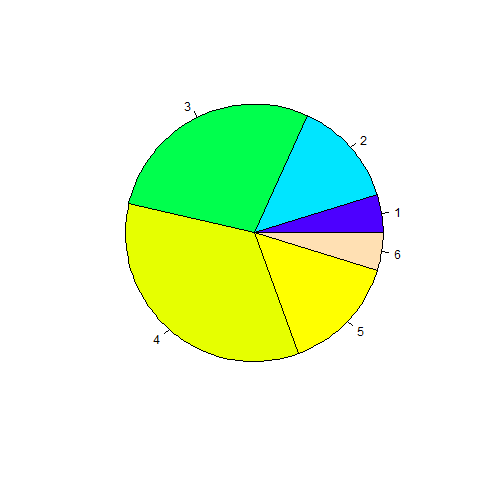
\includegraphics[height=6cm]{../fig/Cap01-DiagramaSectores.png}
% 	\hspace{0.5cm}
	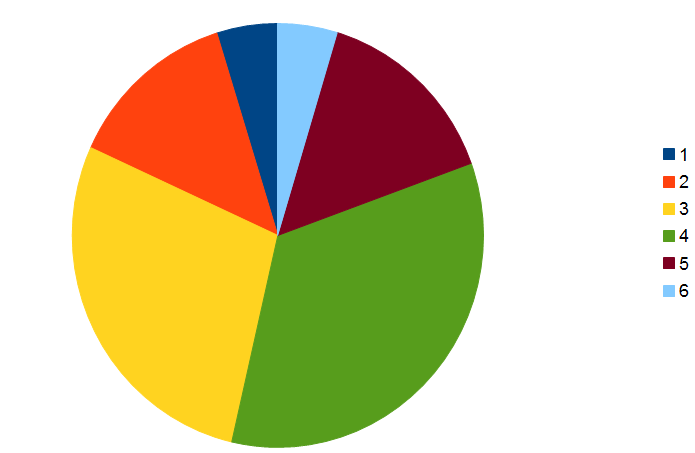
\includegraphics[height=7cm]{../fig/Cap01-DiagramaSectoresconCalc.png}
	\end{enColor}
	\begin{bn}
% 	\includegraphics[height=6cm]{../fig/Cap01-DiagramaSectores-bn.png}
% 	\hspace{0.5cm}
	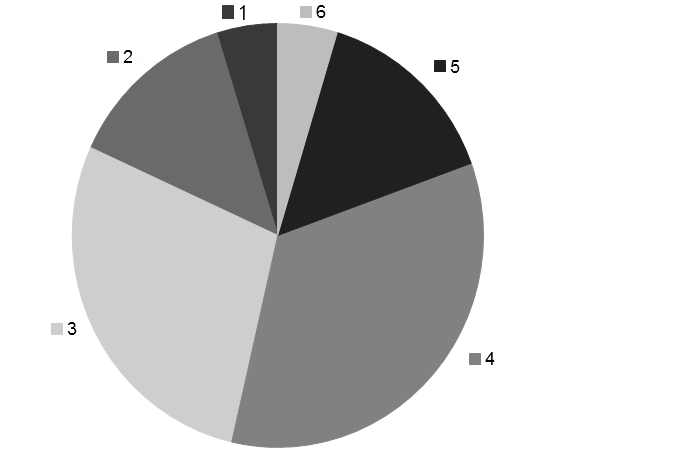
\includegraphics[height=7cm]{../fig/Cap01-DiagramaSectoresconCalc-bn.png}
	\end{bn}
	\caption{Diagrama de sectores circulares, dibujado con Calc.}
	\label{cap01:fig:DiagramaSectores}
    \end{figure}

Los \index{diagrama de barras o columnas} {\sf diagramas de barras o columnas}\index{barras, diagrama de }\index{columnas, diagrama de} tienen,
  en general, más precisión que los de sectores. En la parte (a) de la Figura
  \ref{cap01:fig:DiagramaBarras} se muestra el mismo conjunto de valores que antes vimos en el diagrama de sectores. Y ahora es evidente que, aunque
  son muy parecidas, la frecuencia del valor 2 es menor que la del valor 5. Además, los diagramas de barras se pueden utilizar para  mostrar varios conjuntos de datos simultáneamente, facilitando la comparación entre ellos, como en la parte (b) de la Figura  \ref{cap01:fig:DiagramaBarras}.
  \begin{figure}[phtb]
	\begin{center}
	\begin{enColor}
    (a)\\
	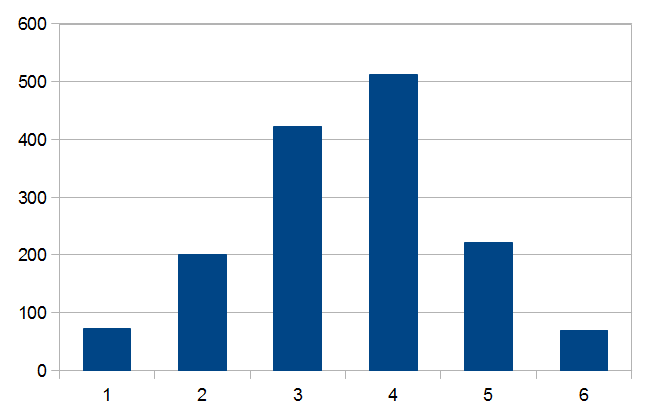
\includegraphics[width=10cm]{../fig/Cap01-DiagramaBarrasconCalc.png}\\[3mm]
    (b)\\
    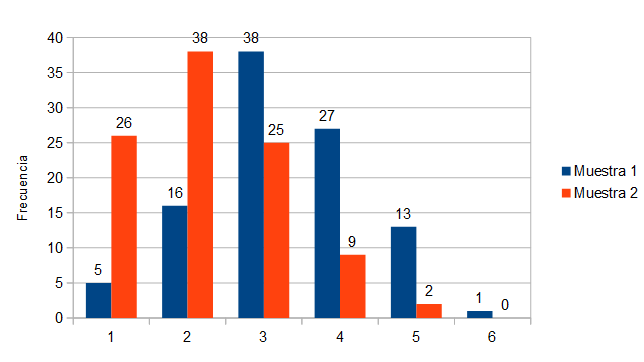
\includegraphics[width=10cm]{../fig/Cap01-DiagramaBarrasDosMuestras.png}\\[3mm]
	\end{enColor}
	\begin{bn}
    (a)\\
	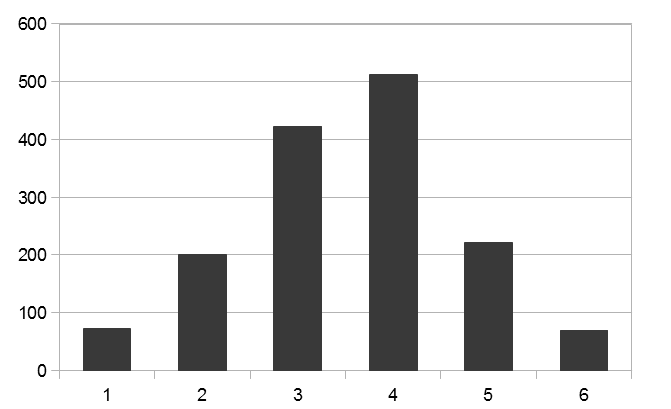
\includegraphics[width=10cm]{../fig/Cap01-DiagramaBarrasconCalc-bn.png}\\[3mm]
    (b)\\
    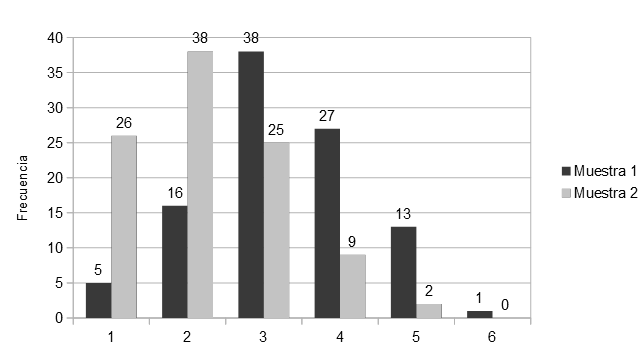
\includegraphics[width=10cm]{../fig/Cap01-DiagramaBarrasDosMuestras-bn.png}\\[3mm]
	\end{bn}
	\caption{Diagrama de barras para (a) un conjunto de datos, (b) dos conjuntos de datos.}
	\label{cap01:fig:DiagramaBarras}
    \end{center}
  \end{figure}

En los tutoriales aprenderemos a dibujar este tipo de gráficos.

%
\subsection{Histogramas.}
\label{cap01:sec:Histogramas}

Un {\sf histograma} \index{histograma}  es un tipo especial de
diagrama   de barras que se utiliza para variables cuantitativas agrupadas en
intervalos (clases) (recuerda la discusión que precedía a la Tabla \ref{cap01:tabla:FrecuenciaPesoClase}, pág.
\pageref{cap01:tabla:FrecuenciaPesoClase}). Puedes ver un ejemplo en la Figura \ref{cap01:fig:Histograma}. Las
dos  propiedades básicas que caracterizan a un histograma son:
    \begin{enumerate}
      \item Las {\em bases de cada una de las barras se corresponden con
      los intervalos} en los que hemos dividido el recorrido de los valores de la
      variable continua.

      \item El {\em área de cada barra es proporcional a la
      frecuencia  correspondiente a ese intervalo.}
    \end{enumerate}

\begin{figure}[h]
\centering
\begin{enColor}
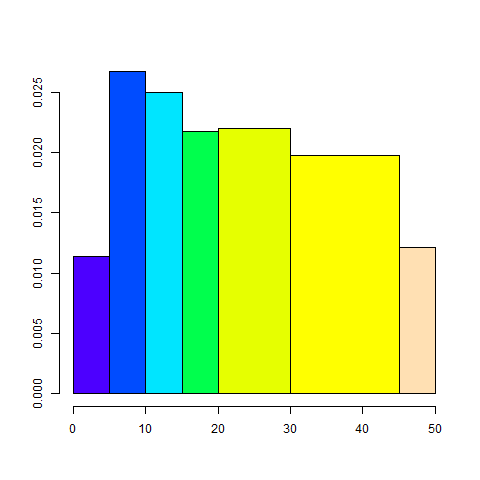
\includegraphics[height=7cm]{../fig/Cap01-Histograma.png}
\end{enColor}
\begin{bn}
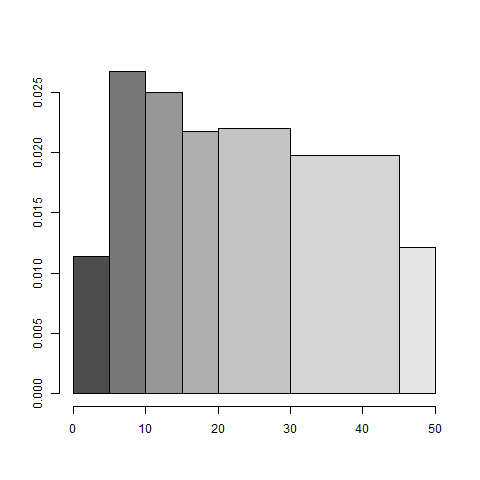
\includegraphics[height=7cm]{../fig/Cap01-Histograma-bn.png}
\end{bn}
\caption{Histograma.}
\label{cap01:fig:Histograma}
\end{figure}

Una consecuencia de estas propiedades es que las columnas de un histograma no tienen porque tener la misma anchura, como se ve en la Figura
\ref{cap01:fig:Histograma}.

Dos observaciones adicionales: en primer lugar, puesto que los
intervalos deben cubrir todo el recorrido de la variable, en un histograma no
hay espacio entre las barras. Y, como práctica recomendable, para que la
visualización sea efectiva, no es conveniente utilizar un histograma con más de
10 o 12 intervalos, ni con menos de cinco o seis.

En el caso de {\sf variables cuantitativas discretas}, normalmente los
intervalos se extienden a valores intermedios (que la variable no puede
alcanzar) para que no quede espacio entre las barras del histograma.

Los pasos para obtener el histograma, en el caso en el que todos los intervalos son de la misma longitud, son estos:
\begin{enumerate}

      \item Si no nos los dan hechos, debemos empezar por determinar los
      intervalos.  Para ello podemos localizar el valor máximo y el mínimo de
      los valores, restarlos y obtenemos el {\em recorrido} de la variable (daremos más detalles en el Capítulo \ref{cap:ValoresCentralesDispersion}).

      \item Dividimos ese recorrido entre el número de intervalos deseados,	
      para obtener la longitud de cada uno de los intervalos. Construimos los
      intervalos y la tabla de frecuencias correspondiente.

      \item Calculamos la altura de cada barra, teniendo en cuenta que
      área=base$\cdot$ altura, y que el área ({!`}no la altura!) es proporcional a
      la frecuencia. Por lo tanto podemos usar:

%      \begin{center}
%        \fbox{\colorbox{Gris025}{
%          \begin{minipage}{8cm}
%	    \[
%	      \mbox{altura}=\dfrac{\mbox{frecuencia}}{\mbox{base}}=\dfrac{\mbox{frecuencia del intervalo}}
%	      {\mbox{anchura del intervalo}}
%	    \]
%          \end{minipage}}
%        }
%     \end{center}
        \begin{center}
                \fcolorbox{black}{Gris025}{\begin{minipage}{8cm}	    \[
        	      \mbox{altura}=\dfrac{\mbox{frecuencia}}{\mbox{base}}=\dfrac{\mbox{frecuencia del intervalo}}
        	      {\mbox{longitud del intervalo}}
        	    \]
        \end{minipage}}
        \end{center}
para calcular la altura de cada una de las barras.
\end{enumerate}
Quizá la mejor manera de entender la propiedad más importante (y más útil) de un histograma sea viendo un {\em falso histograma}, un histograma mal hecho.
\begin{ejemplo}
\label{cap01:ejem:HistogramaMalHecho}
En la Tabla \ref{cap01:tabla:EjemploHistogramaMalHecho} se muestra la tabla de frecuencia de un conjunto de datos, agrupados por intervalos (clases). Observa que la longitud del último intervalo, el intervalo $(8,12]$, es el doble de las longitudes de los restantes intervalos, que son todos de longitud $2$.

\begin{table}[ht]
\centering
\begin{tabular}{|l|rrrrr|}
  \hline
Clase & [0,2] & (2,4] & (4,6] & (6,8] & (8,12] \\
  \hline
Frecuencia & 1320 & 3231 & 1282 & 900 & 1105 \\
   \hline
\end{tabular}
\caption{Datos para el Ejemplo \ref{cap01:ejem:HistogramaMalHecho}}
\label{cap01:tabla:EjemploHistogramaMalHecho}
\end{table}

En la parte (a) de la Figura \ref{cap01:fig:Histograma} se muestra un falso histograma, en el que la altura de las columnas se corresponde con esas frecuencias. Para un observador que no disponga de la Tabla \ref{cap01:tabla:EjemploHistogramaMalHecho} (e incluso si dispone de ella, en muchos casos), la sensación que transmite ese gráfico es que el número de casos que corresponden al intervalo $(8,12]$ es mucho mayor que los del intervalo $(6,8]$. Resulta poco claro, en esta representación gráfica, el hecho relevante de que esa frecuencia mayor se corresponde con un intervalo el doble de ancho. El sistema perceptivo humano tiende a dar más importancia a las figuras con mayor área, especialmente si sus alturas son parecidas.

\begin{figure}[hbpt]
\centering
\begin{enColor}
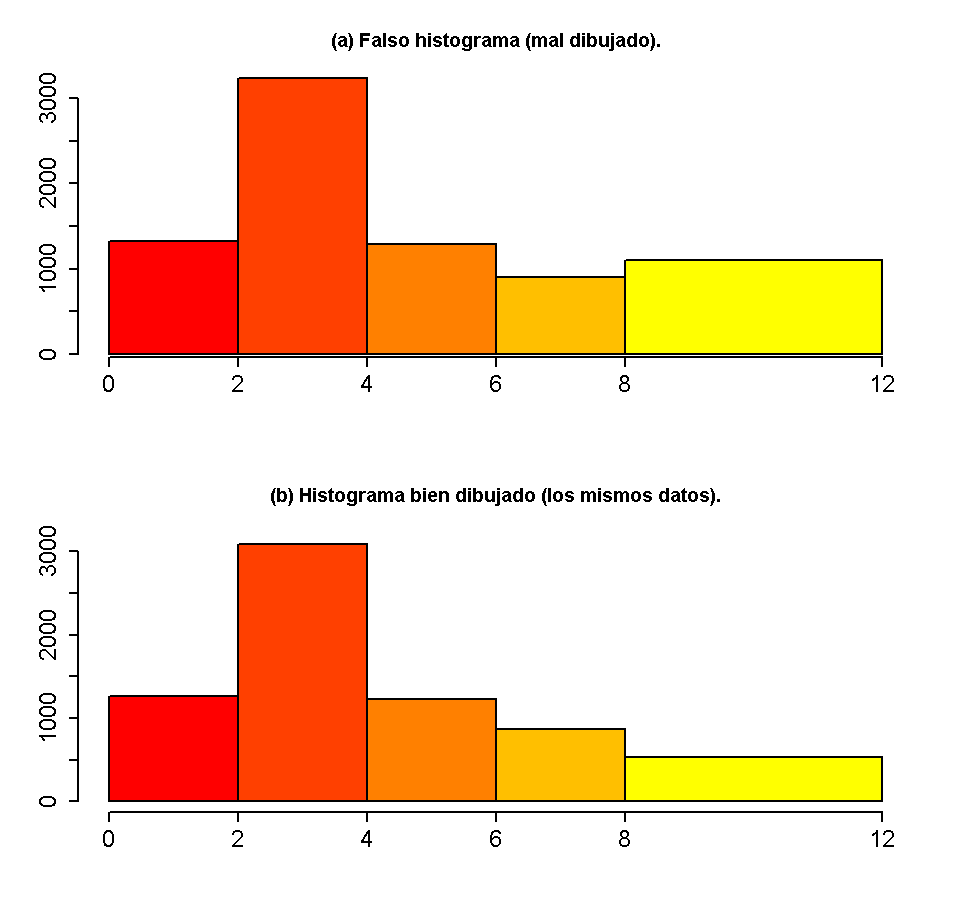
\includegraphics[width=12cm]{../fig/Cap01-HistogramaMalHecho.png}
\end{enColor}
\begin{bn}
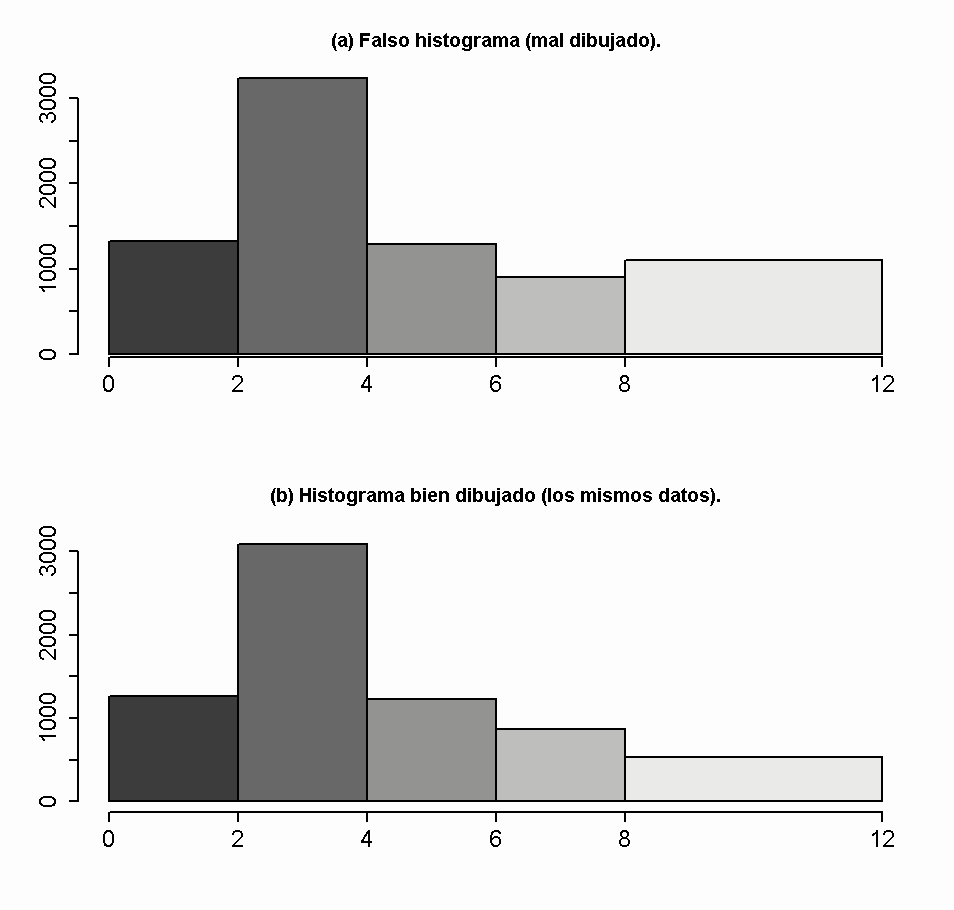
\includegraphics[width=12cm]{../fig/Cap01-HistogramaMalHecho-bn.png}
\end{bn}
\caption{Representación de los datos del Ejemplo \ref{cap01:ejem:HistogramaMalHecho}, con un (a) falso histograma (con {\em la altura} proporcional a la frecuencia), y (b) el histograma correcto para esos mismos datos (con {\em el área} proporcional a la frecuencia).}
\label{cap01:fig:Histograma}
\end{figure}
\end{ejemplo}

En la parte (b) de esa Figura, por otra parte, aparece el histograma correctamente dibujado. Como puede apreciarse, el hecho de hacer que sea el área de la columna lo que se corresponda con la frecuencia, ayuda a captar visualmente la importancia relativa del intervalo $(8,12]$. De esta manera queda de manifiesto que la anchura de ese intervalo es distinta de las otras, sin sobrevalorar la frecuencia que le corresponde.
\qed

%    \item Pronto aprenderemos a obtener muchos de los resultados de este
%capítulo usando R. Como aperitivo, aquí tenemos un
%\textattachfile{Sesion001.R}{\textcolor{blue}{fichero}} de instrucciones para el
%ejemplo que hemos usado hoy.


%\Pendiente{TODO NUEVO}
\section{Precisión y exactitud. Cifras significativas.}
\label{cap01:sec:PrecisionExactitudCifrasSignificativas}

Vamos a aprovechar la sección final de este capítulo para introducir algunas herramientas de lenguaje, y procedimientos de trabajo con datos
numéricos que usaremos a lo largo de todo el libro. Hemos repetido varias veces en este capítulo que la diferencia entre variables cuantitativas discretas y continuas es bastante sutil. En particular, en el caso de datos agrupados en clases (ver el apartado
\ref{cap01:subsec:NotacionVariablesTablasFrecuenciaDatosAgrupados} y especialmente la discusión de la pág. \pageref{cap01:tabla:FrecuenciaPesoClase}),
surge la pregunta de cómo definir el límite entre dos clases. Aunque en los tutoriales veremos cómo hacer esto en la práctica, podemos preparar el terreno. Esta cuestión, a su vez, está estrechamente ligada a la cuestión de las unidades de medida
que se utilizan, y de la precisión con la que obtenemos esas medidas. Volviendo al ejemplo de los alumnos de una clase, es muy extraño pensar que
alguien nos va a decir que uno de esos alumnos pesa 65.2365789 kilogramos. ¿De verdad nos creemos que tiene sentido expresar así el peso de una
persona, cuando la pérdida de un sólo cabello\footnote{Una persona tiene aproximadamente cien mil pelos en la cabeza, cada uno de unos miligramos de peso.} cambiaría esa cifra en una
escala mucho mayor que la supuesta ``precisión'' de la medida? Naturalmente que no. Por esa razón, al hablar del peso de una persona lo más
{\em práctico} es trabajar en kilos, a lo sumo en cientos o decenas de gramos. Al hacer esto, sucede algo interesante: si usamos los kilos como
unidad de medida, sin preocuparnos de diferencias más finas, diremos que un alumno pesa 57 kilos y otro 58 kilos, pero no diremos nunca que pesa 55'5
o 55'32 kilos. Es decir, que al trabajar de esa manera, estaremos usando el peso {\em como si fuera una variable discreta}, que cambia a saltos, de
kilo en kilo. El lector estará pensando {!`}pero el peso \underline{ES} continuo! Y lo que queremos es invitarle a descubrir que el peso no es ni
continuo ni discreto. En distintos problemas usamos distintos modelos, y matemáticas distintas, para trabajar con las medidas de peso. Y la decisión
sobre cuál es el modelo más adecuado depende muchas veces de la precisión y exactitud con las que deseamos trabajar.

Aprovechemos la ocasión para establecer una distinción entre las nociones de precisión y exactitud. Aunque a menudo se usan indistintamente en el
lenguaje cotidiano\footnote{El Diccionario de la Real Academia Española (ver enlace [\,\ref{enlace0000-2}\,]\label{enlace0000a-2}) nos
parece especialmente poco atinado en estas dos entradas...}, estas dos nociones tienen significados técnicos distintos. No queremos entrar en una
discusión demasiado técnica, así que vamos a recurrir, para ilustrar la diferencia entre ambas nociones a la imagen, que se usa a menudo de una diana
a la que estamos tratando de acertar. La idea se ilustra en la Figura \ref{cap01:fig:PrecisionExactitud} (pág.
\pageref{cap01:fig:PrecisionExactitud}). Como puede verse, la idea de precisión se
relaciona con la distancia al objetivo (con el tamaño del error que se comete, visto de otra manera.)  En cambio, la idea de exactitud tiene que ver
con la posición de nuestros disparos, y con el hecho de que esos disparos estén {\em centrados} en el blanco.
    \begin{figure}[h]
	\centering
	\begin{enColor}
% 	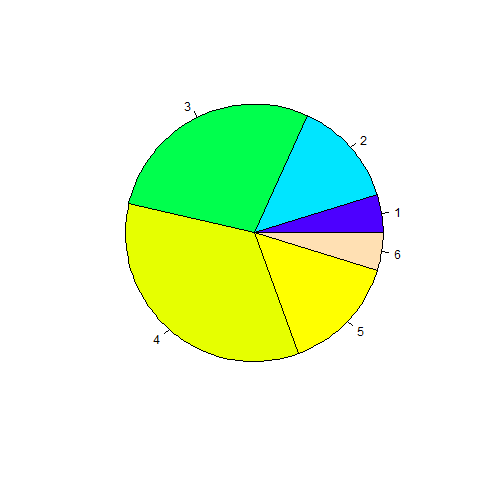
\includegraphics[height=6cm]{../fig/Cap01-DiagramaSectores.png}
% 	\hspace{0.5cm}
	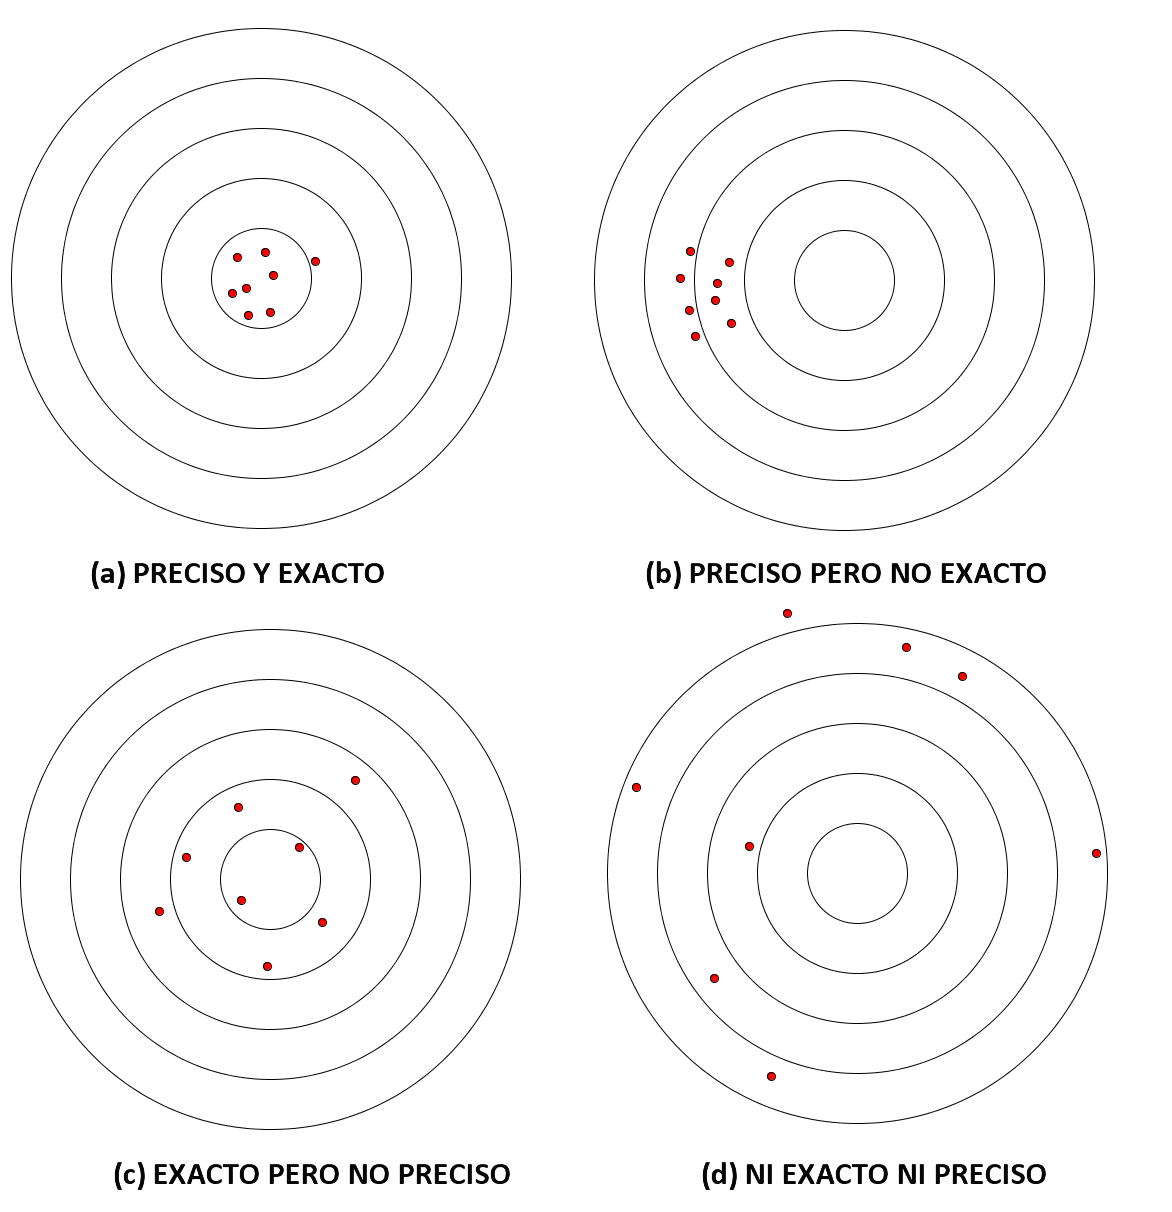
\includegraphics[width=10cm]{../fig/Cap01-PrecisionExactitud-2.png}
	\end{enColor}
	\begin{bn}
% 	\includegraphics[height=6cm]{../fig/Cap01-DiagramaSectores-bn.png}
% 	\hspace{0.5cm}
	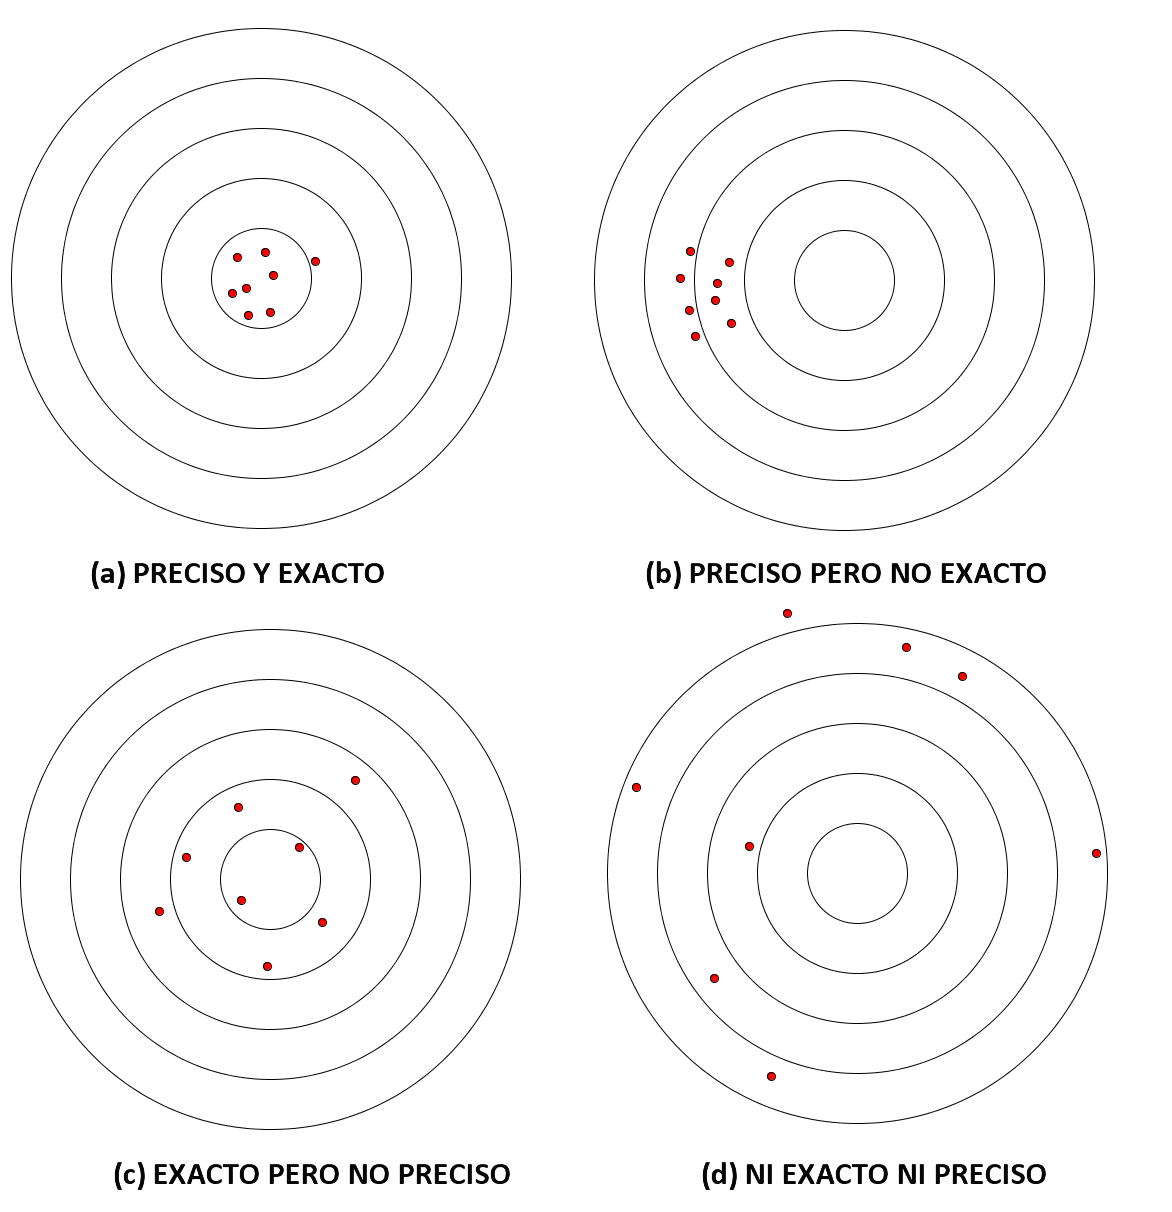
\includegraphics[width=10cm]{../fig/Cap01-PrecisionExactitud-2.png}
	\end{bn}
	\caption{Precisión y exactitud.}
	\label{cap01:fig:PrecisionExactitud}
    \end{figure}

A lo largo del curso, y muy especialmente en el próximo capítulo, vamos a tener sobradas ocasiones de volver sobre estas dos ideas. Pero ya que
vamos a trabajar muy a menudo con valores numéricos, vamos a hablar del concepto de {\sf cifras significativas}\index{cifras significativas}, que está
muy relacionado con la idea de precisión de las medidas.

Todos los números que proceden de mediciones tienen una precisión limitada, ligada a menudo al propio aparato o proceso de medición. Por ejemplo, y
para que no suene muy abstracto, si medimos una longitud con una regla típica, la precisión de la medida sólo llega al milímetro, porque esas son las
divisiones de la escala en nuestra regla. De la misma forma un termómetro doméstico no suele afinar más allá de las décimas de grado, la balanza de
cocina distingue normalmente, a lo sumo, gramos, etcétera.

Por esa razón, si hemos medido con la regla una longitud de 5cm, o sea 50mm, y lo hemos hecho teniendo cuidado de precisar hasta el milímetro, sabemos
que en realidad sólo hemos sido capaces de asegurar que el valor de la longitud está entre
\[50-1=49,\qquad\mbox{ y }\qquad 50+1=51\mbox{ mm.}\]
Hasta aquí las cosas son relativamente fáciles. El problema viene, habitualmente, cuando se hacen operaciones con los resultados de las medidas. Por
ejemplo, si dividimos esa longitud en tres trozos iguales, ¿cuánto medirán esos tres trozos? Si tecleamos en una calculadora $50/3$ podemos terminar
respondiendo algo como que esos trozos miden:
\[16.66666667\mbox{ mm.}\]
Así, mediante el procedimiento mágico de aporrear las teclas de una calculadora, resulta que una medida que sólo conocíamos con una precisión de un
milímetro se ha convertido en un resultado preciso casi hasta la escala atómica. Evidentemente esta no es la forma correcta de trabajar. Es necesario
algún proceso de {\sf redondeo}\index{redondeo, cifras significativas} para obtener un resultado preciso.

Uno de los objetivos secundarios de este curso es proporcionar al lector una formación básica en el manejo de los números como instrumentos de
comunicación científica. Vamos a empezar, en este apartado, por familiarizarnos con la noción de cifras significativas, y poco a poco, en sucesivas
visitas a este tema, iremos aprendiendo cómo se manejan correctamente situaciones como la que hemos descrito, en la que hacemos operaciones con
números aproximados. Trataremos, también en esto, de darle un enfoque siempre eminentemente práctico a lo que hagamos.

Así que, en lugar de empezar tratando de definir qué son las cifras significativas, comencemos con algunos ejemplos, para ilustrar la forma de proceder. La idea intuitiva, en cualquier caso, es buscar el número con una cierta cantidad de cifras más cercano al número de partida. Precisar esta idea requiere tener en cuenta varios detalles técnicos intrincados, pero como ilustran los siguientes ejemplos el resultado es un procedimiento mecánico muy sencillo de aplicar.

\begin{Ejemplo}
Supongamos que nos dan el número
\[1.623698\]
y nos piden que lo redondeemos a cuatro cifras significativas. Se trata, por tanto, de aprender a redondear un número dado, en notación decimal, a una cierta cantidad de cifras significativas (cuatro, en este ejemplo). El procedimiento es
este:
\begin{enumerate}
  \item empezando desde la primera cifra del número (la situada más a la izquierda), buscamos la primera cifra que no sea un cero. En el ejemplo esa cifra es $1$, la primera del número por la izquierda.
  \[
    \begin{array}{cccccccc}
      \mathbf{1}&.&6&2&3&6&9&8\\
      \mathbf{\uparrow}\\
    \end{array}
  \]
  Para este paso no importa la posición del punto decimal. La única duda que se puede plantear es si hay ceros a la izquierda, y ese caso lo veremos enseguida, más abajo.
  \item Como queremos cuatro cifras significativas, empezamos a contar desde esa primera cifra (inclusive) hacia la derecha, hasta llegar a  cuatro cifras.
  \[
    \begin{array}{cccccccc}
      1&.&6&2&3&6&9&8\\
      \mathbf{\uparrow}&&\mathbf{\uparrow}&\mathbf{\uparrow}&\mathbf{\uparrow}\\
      1^o&&2^o&3^o&4^o
    \end{array}
  \]
  \item Ahora miramos la siguiente cifra, en este caso la quinta (que es un seis). Y aplicamos esta regla de decisión: si la quinta cifra es mayor o igual que 5, sumamos 1 a la cuarta cifra, con acarreo si es necesario (veremos esto en el siguiente ejemplo). En el ejemplo,
  \[
    \begin{array}{cccccccc}
      1&.&6&2&3&\mathbf{6}&9&8\\
      &&&&&\mathbf{\uparrow}\\
      &&&&&5^o
    \end{array}
  \]
  Como la quinta cifra es 6, y por lo tanto mayor o igual a 5,  sumamos 1 a la última cifra de 1.623 (las cuatro primeras cifras no nulas del número original) y obtenemos:
  \[1.62\mathbf{4}.\]
  Este es el valor de $1.623698$ redondeado a cuatro cifras significativas.
  \end{enumerate}

  Veamos ahora un ejemplo más complicado, en el que entran en juego reglas adicionales de redondeo. De nuevo nos dan un número, en este caso
  \[0.00337995246\]
  y vamos a redondearlo, ahora a cinco cifras significativas. Aplicamos el mismo esquema:
  \begin{enumerate}
  \item Empezando desde la primera cifra del número (la situada más a la izquierda), buscamos la primera cifra que no sea un cero. En el ejemplo esa cifra es $3$, en realidad la cuarta cifra del número por la izquierda (la tercera después del punto decimal).
  \[
    \begin{array}{cccccccccccccc}
      0&.&0&0&\mathbf{3}&3&7&9&9&5&2&4&6\\
      &&&&\mathbf{\uparrow}\\
    \end{array}
  \]
  Los ceros a la izquierda no se tienen en cuenta para el total de cifras significativas.
  \item Como queremos cinco cifras significativas, empezamos a contar desde el 3 que hemos localizado en el paso anterior, y  hacia la derecha, hasta llegar a  cinco cifras.
  \[
    \begin{array}{cccccccccccccc}
      0&.&0&0&\mathbf{3}&\mathbf{3}&\mathbf{7}&\mathbf{9}&\mathbf{9}&5&2&4&6\\
      &&&&\mathbf{\uparrow}&\mathbf{\uparrow}&\mathbf{\uparrow}&\mathbf{\uparrow}&\mathbf{\uparrow}\\
      &&&&1^o&2^o&3^o&4^o&5^o
    \end{array}
  \]
  \item Miramos la siguiente cifra, que en este caso es un cinco.
  \[
    \begin{array}{cccccccccccccc}
      0&.&0&0&{3}&{3}&{7}&{9}&{9}&\mathbf{5}&2&4&6\\
      &&&&&&&&&\mathbf{\uparrow}\\
    \end{array}
  \]
  Como esa cifra es mayor o igual a 5,  sumamos 1 a la última cifra de $0.0033799$ (la parte precedente del número original) y obtenemos:
  \[0.0033800.\]
  Fíjate en que hemos hecho la suma con acarreo (dos acarreos, porque había dos nueves al final). Y que, al hacer esto, conservamos los ceros que aparecen a la derecha. Es importante hacer esto, porque esos ceros sí que son cifras significativas (a diferencia de los ceros de la izquierda, que no cuentan).
  Así que el número, redondeado a cinco cifras significativas es $0.0033800$.

  Un último ejemplo. Hasta ahora, en los dos ejemplos que hemos visto, el proceso de redondeo ocurría a la derecha del punto decimal. Pero si nos
  piden que redondeemos el número $324755$ a tres cifras significativas, acabaremos con el número $325000$. Los ceros a la derecha son, en este caso,
  imprescindibles. Este último ejemplo pretende ayudar a clarificar un hecho básico: el proceso de redondeo a cifras significativas, {\em nunca} afecta a la
  posición de la coma decimal en el número.  \flushright$\Box$
\end{enumerate}
\end{Ejemplo}
Naturalmente, esta receta no agota la discusión, ni mucho menos. Para empezar, no hemos dicho nada sobre la forma de {\em operar} con números aproximados. Si tengo dos números con cuatro cifras significativas y los multiplico, ¿cuántas cifras significativas tiene el producto? ¿Y qué sucede si calculo la raíz cuadrada de un número con tres cifras significativas?  Veamos un ejemplo sencillo, para que el lector comprenda de que se trata:
\begin{ejemplo}
Tenemos los dos números
\[\begin{cases}
a= 10000\\
b= 2.1
\end{cases}\]
y suponemos que los dos tienen dos cifras significativas, que se han redondeado usando el procedimiento que hemos descrito. En el caso de $a$, y con las reglas de redondeo que hemos dado esto significa que sólo podemos asegurar que $a$ cumple:
\[10000-499< a < 10000+499 \]
Y en particular, al calcular la suma $a+b$ no tiene ningún sentido decir que es
\[a+b=10002.1\]
porque esto parece estar diciendo que conocemos $a+b$ con mucha más precisión de la que conocemos el propio número $a$. Lo razonable en este caso es decir que
\[a+b\approx a\]
donde el símbolo $\approx$ se lee {\em aproximadamente}, e indica el efecto del redondeo. Al sumar, el número $b$ ``ha desaparecido''. En cambio, si multiplicamos, está claro que debe suceder algo como
\[a\cdot b\approx 21000.\]
Y aún pueden suceder cosas peores. Imagínate que tenemos los números
\[\begin{cases}
c= 43.12\\
d= 43.11
\end{cases}\]
ambos con cuatro cifras significativas, y los restamos. ¿Cuántas cifras significativas tiene el resultado? Como puede verse, es necesario algo más de reflexión para operar acertadamente con números aproximados.
\qed
\end{ejemplo}
Este tipo de preguntas tienen su respuesta detallada en una parte de las Matemáticas llamada {\sf Análisis (o Cálculo) Numérico}\index{análisis numérico}\index{numérico, análisis o cálculo}. En general, cada operación con números aproximados supone una pérdida de precisión. Pero aquí no queremos extendernos, y vamos a dejar sin respuesta esas preguntas. Por el momento, nos basta con que el lector comprenda este procedimiento de redondeo a un número de cifras significativas dado. En la práctica, dado que usaremos el ordenador para la mayor parte de las operaciones, vamos a asumir que, en casi todos los casos, la precisión con la que trabaja la máquina es suficiente para compensar la pérdida de precisión asociada a las operaciones que hacemos. A la larga, ese punto de vista se revela como una ingenuidad, pero de momento no necesitamos más.

